\documentclass[compress]{beamer}
\usepackage{ifthen,verbatim}

\title{Effect of Realistic Alignment Scenarios \\ on TeV Di-muons}
\author{Jim Pivarski, Alexei Safonov}
\institute{Texas A\&M University}
\date{ 5 October, 2007}

\newcommand{\isnote}{}
\xdefinecolor{lightyellow}{rgb}{1.,1.,0.25}
\xdefinecolor{darkblue}{rgb}{0.1,0.1,0.7}

%% Uncomment this to get annotations
\def\notes{\addtocounter{page}{-1}
           \renewcommand{\isnote}{*}
	   \beamertemplateshadingbackground{lightyellow}{white}
           \begin{frame}
           \frametitle{Notes for the previous page (page \insertpagenumber)}
           \itemize}
\def\endnotes{\enditemize
	      \end{frame}
              \beamertemplateshadingbackground{white}{white}
              \renewcommand{\isnote}{}}

%% Uncomment this to not get annotations
%% \def\notes{\comment}
%% \def\endnotes{\endcomment}

\setbeamertemplate{navigation symbols}{}
\setbeamertemplate{headline}{\includegraphics[height=1 cm]{../cmslogo} \hspace{0.1 cm} \includegraphics[height=1 cm]{../tamulogo} \hfill
\begin{minipage}{5.5 cm}
\vspace{-0.75 cm} \small
\begin{center}
\ifthenelse{\equal{\insertpagenumber}{1}}{}{\textcolor{blue}{\insertsection}}
\end{center}
\end{minipage} \hfill
\begin{minipage}{4.5 cm}
\vspace{-0.75 cm} \small
\begin{flushright}
\ifthenelse{\equal{\insertpagenumber}{1}}{}{Jim Pivarski \hspace{0.5 cm} \insertpagenumber\isnote/\pageref{numpages}}
\end{flushright}
\end{minipage}\mbox{\hspace{0.2 cm}}}

\begin{document}
\frame{\titlepage}

\begin{frame}
\frametitle{What I've been up to}
\begin{itemize}
\item Developing a track-based muon alignment procedure
\begin{itemize}\setlength{\itemsep}{0.1 cm}
\item Align barrel and endcap in one procedure
\item Based on simple HIP algorithm
\item Two approaches: (a)~stand-alone muons and (b)~globalMuons

(prefer (b), though it introduces tracker $\to$ muon systematics)

\item Currently checking systematic errors; CMS note in production
\end{itemize}

\item Recently applied results of realistically simulated alignments
to TeV di-muons (see yesterday's CSC DPG)

\item We'd like to contribute to TeV di-muon analysis effort

\item The rest of this pdf file is all plots \hfill\textcolor{gray}{(gray is backup)}
\begin{itemize}\setlength{\itemsep}{0.1 cm}
\item Page 3-6: overlays of misaligned di-muon spectra
\item \textcolor{gray}{Page 7-8: event-by-event ratio method for quantifying broadening due to misalignment only}
\item \textcolor{gray}{Page 9-10: applied to individual track momenta, rather than di-muon mass}
\end{itemize}
\end{itemize}
\end{frame}

\begin{frame}
\frametitle{Overlay of \only<1>{1}\only<2>{2} TeV Drell-Yan and $Z'$ resonance}
\begin{columns}
\column{0.5\linewidth}
\only<1>{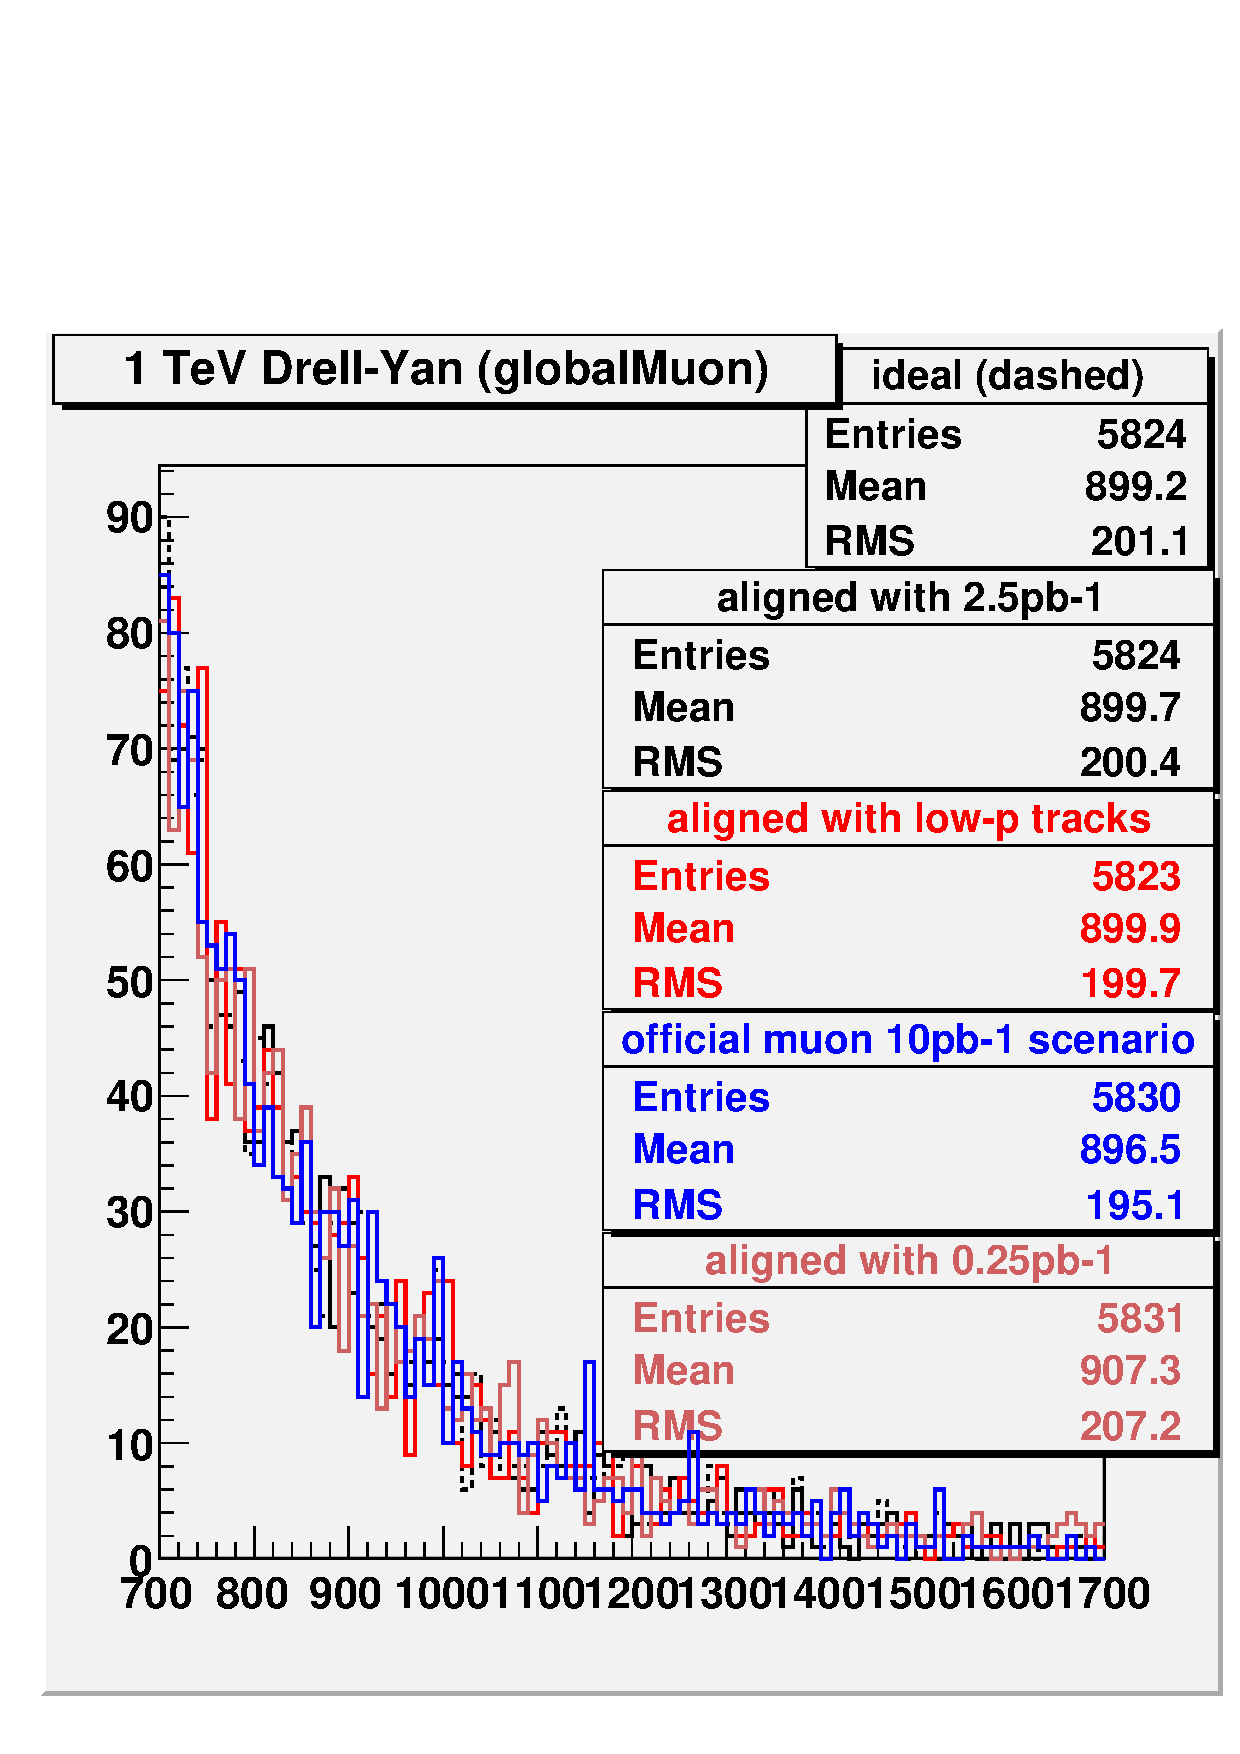
\includegraphics[width=\linewidth]{muoncompare_dy_500.pdf}}
\only<2>{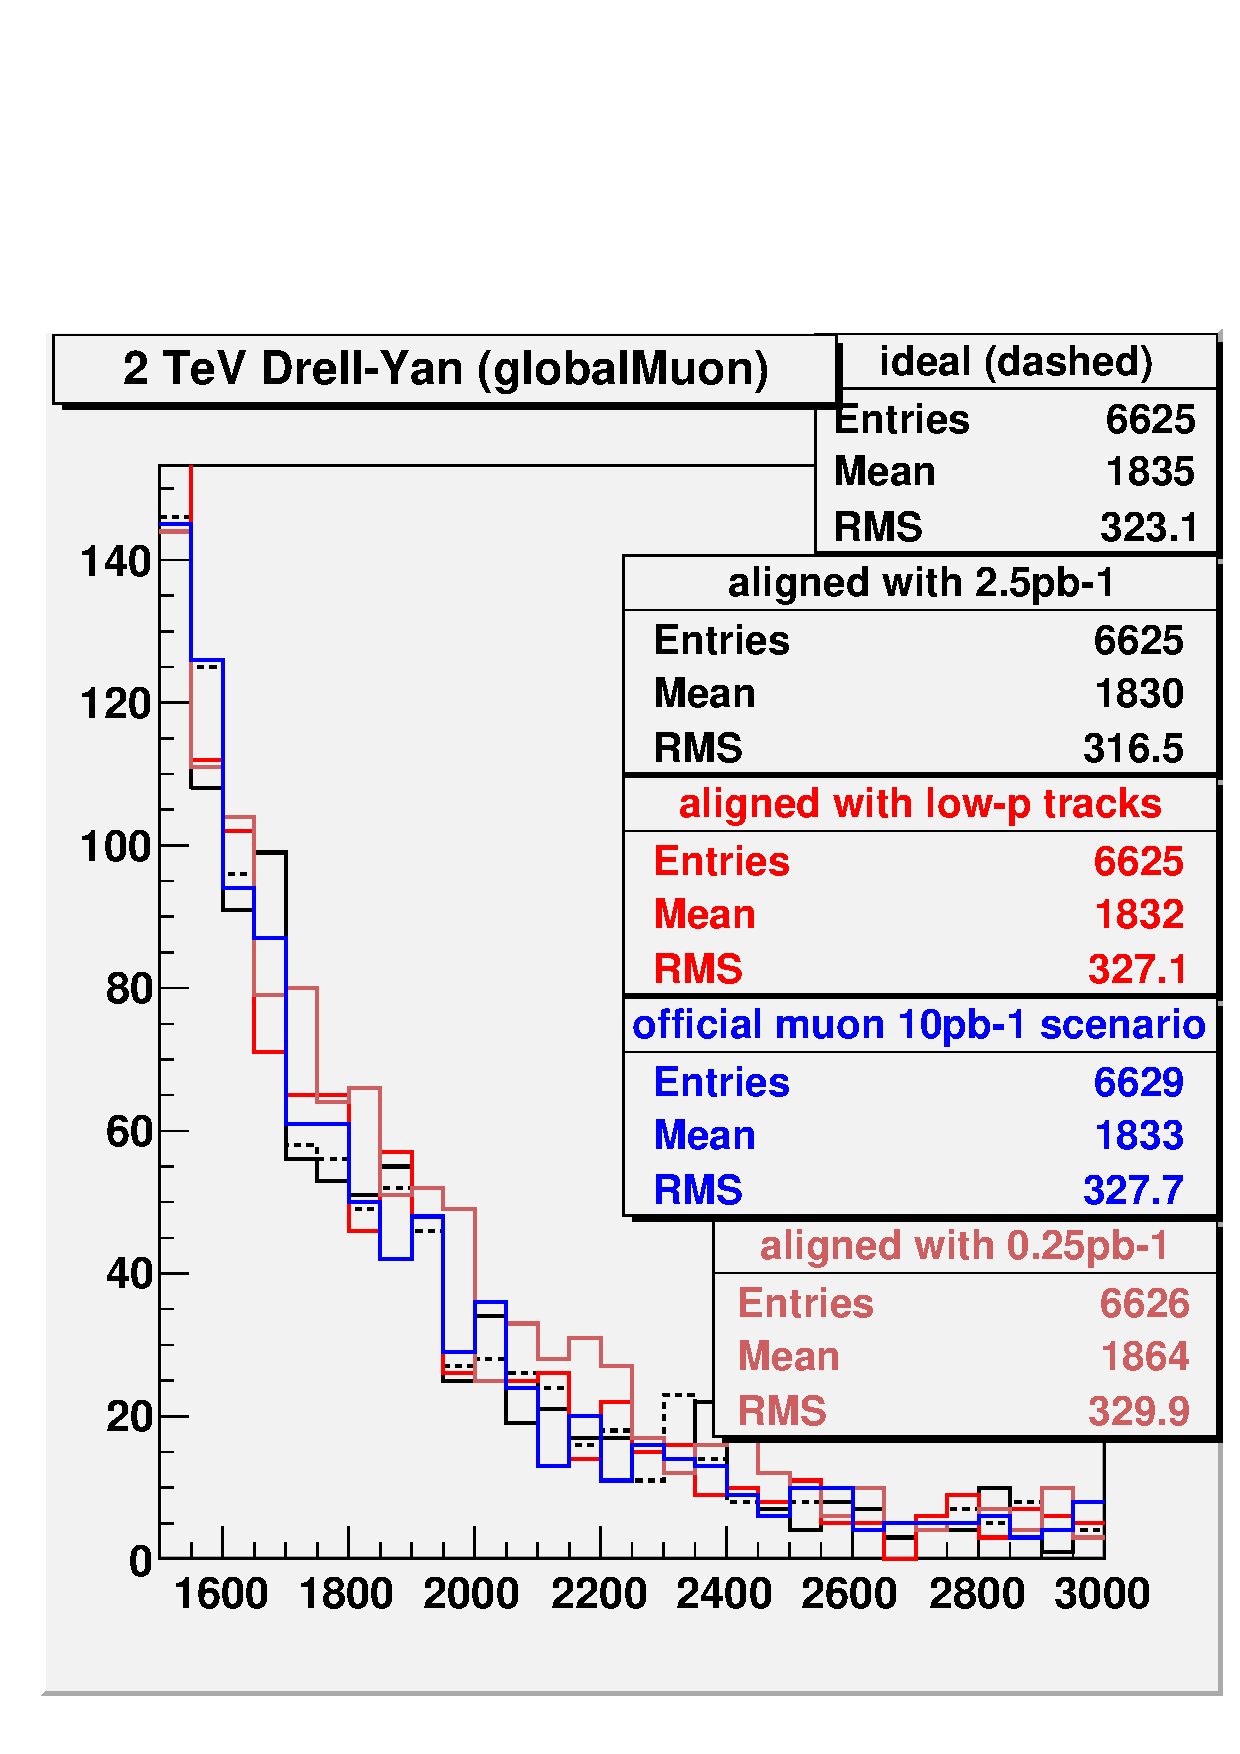
\includegraphics[width=\linewidth]{muoncompare_dy_1000.pdf}}
\column{0.5\linewidth}
\only<1>{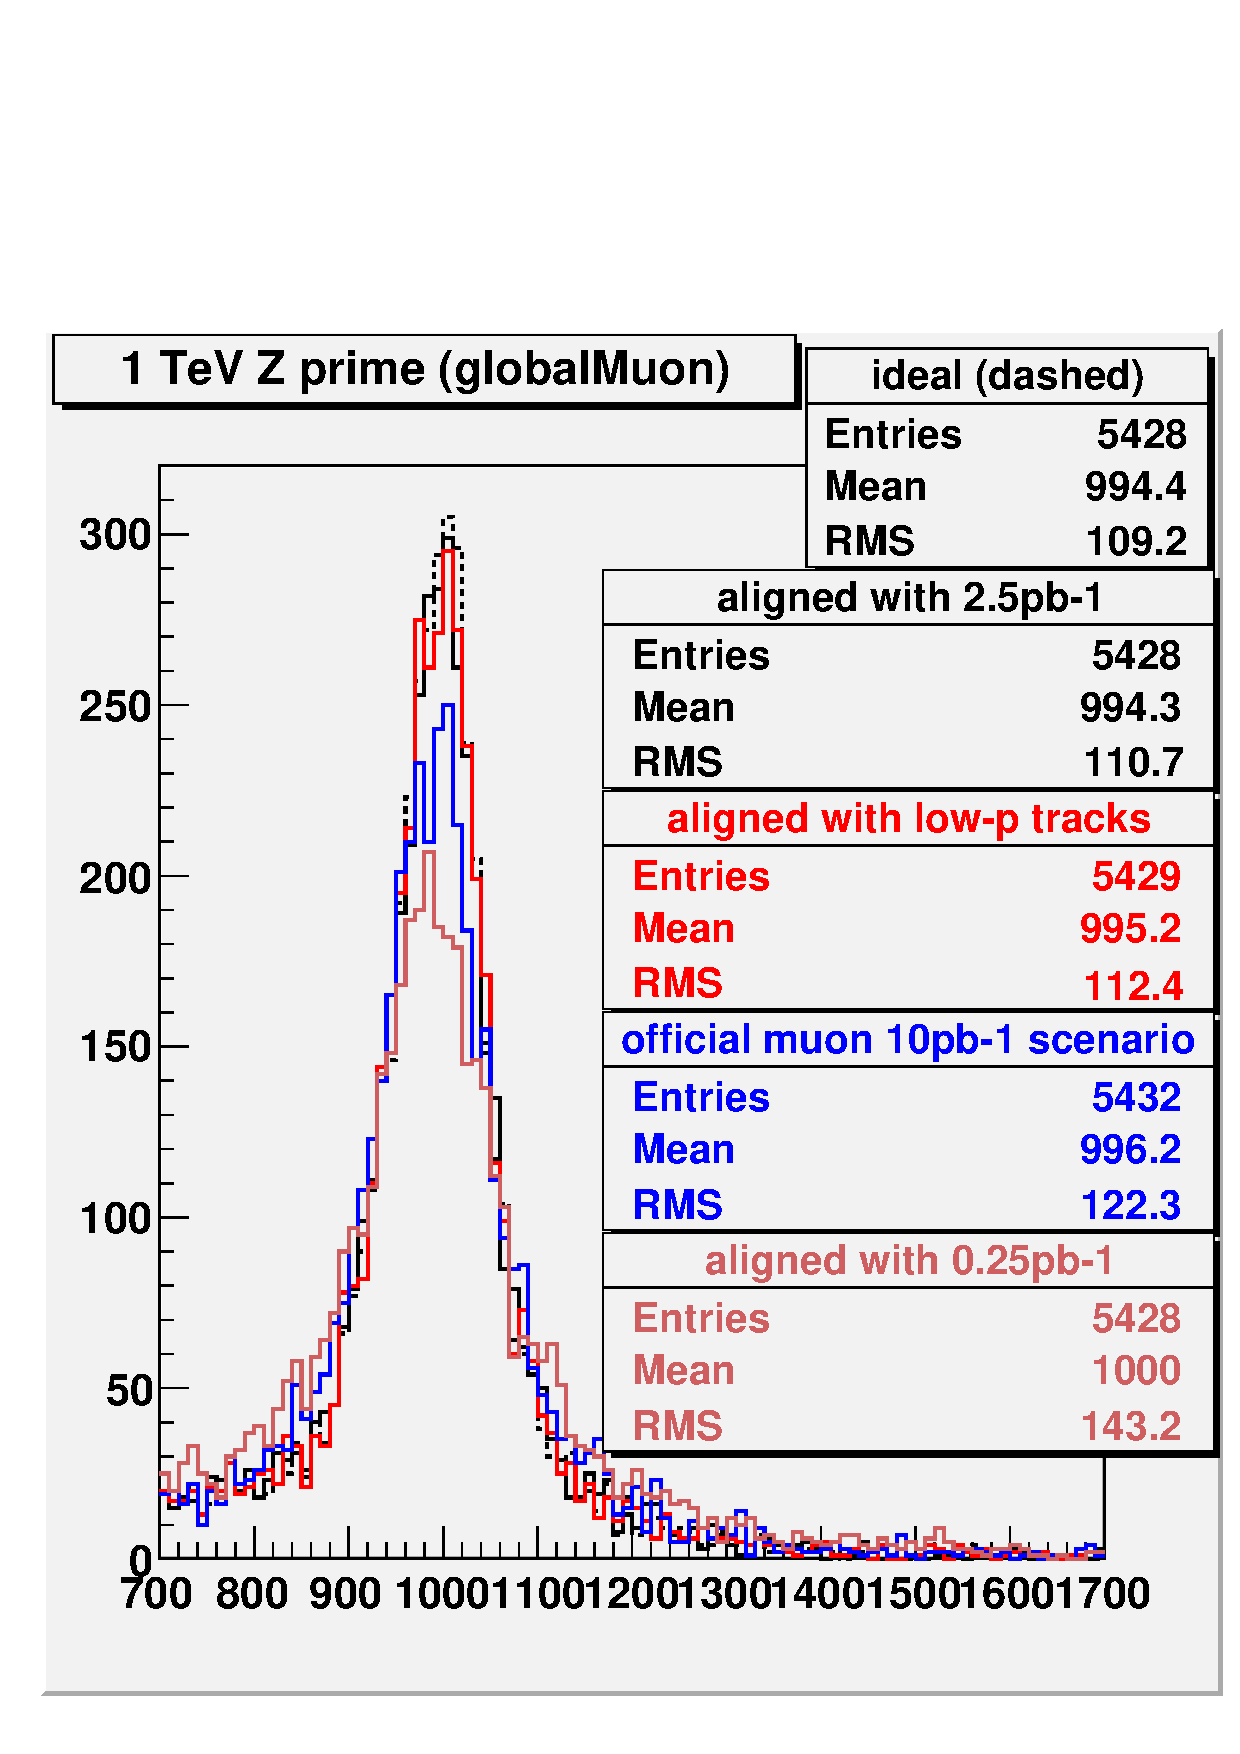
\includegraphics[width=\linewidth]{muoncompare_zprime_1000.pdf}}
\only<2>{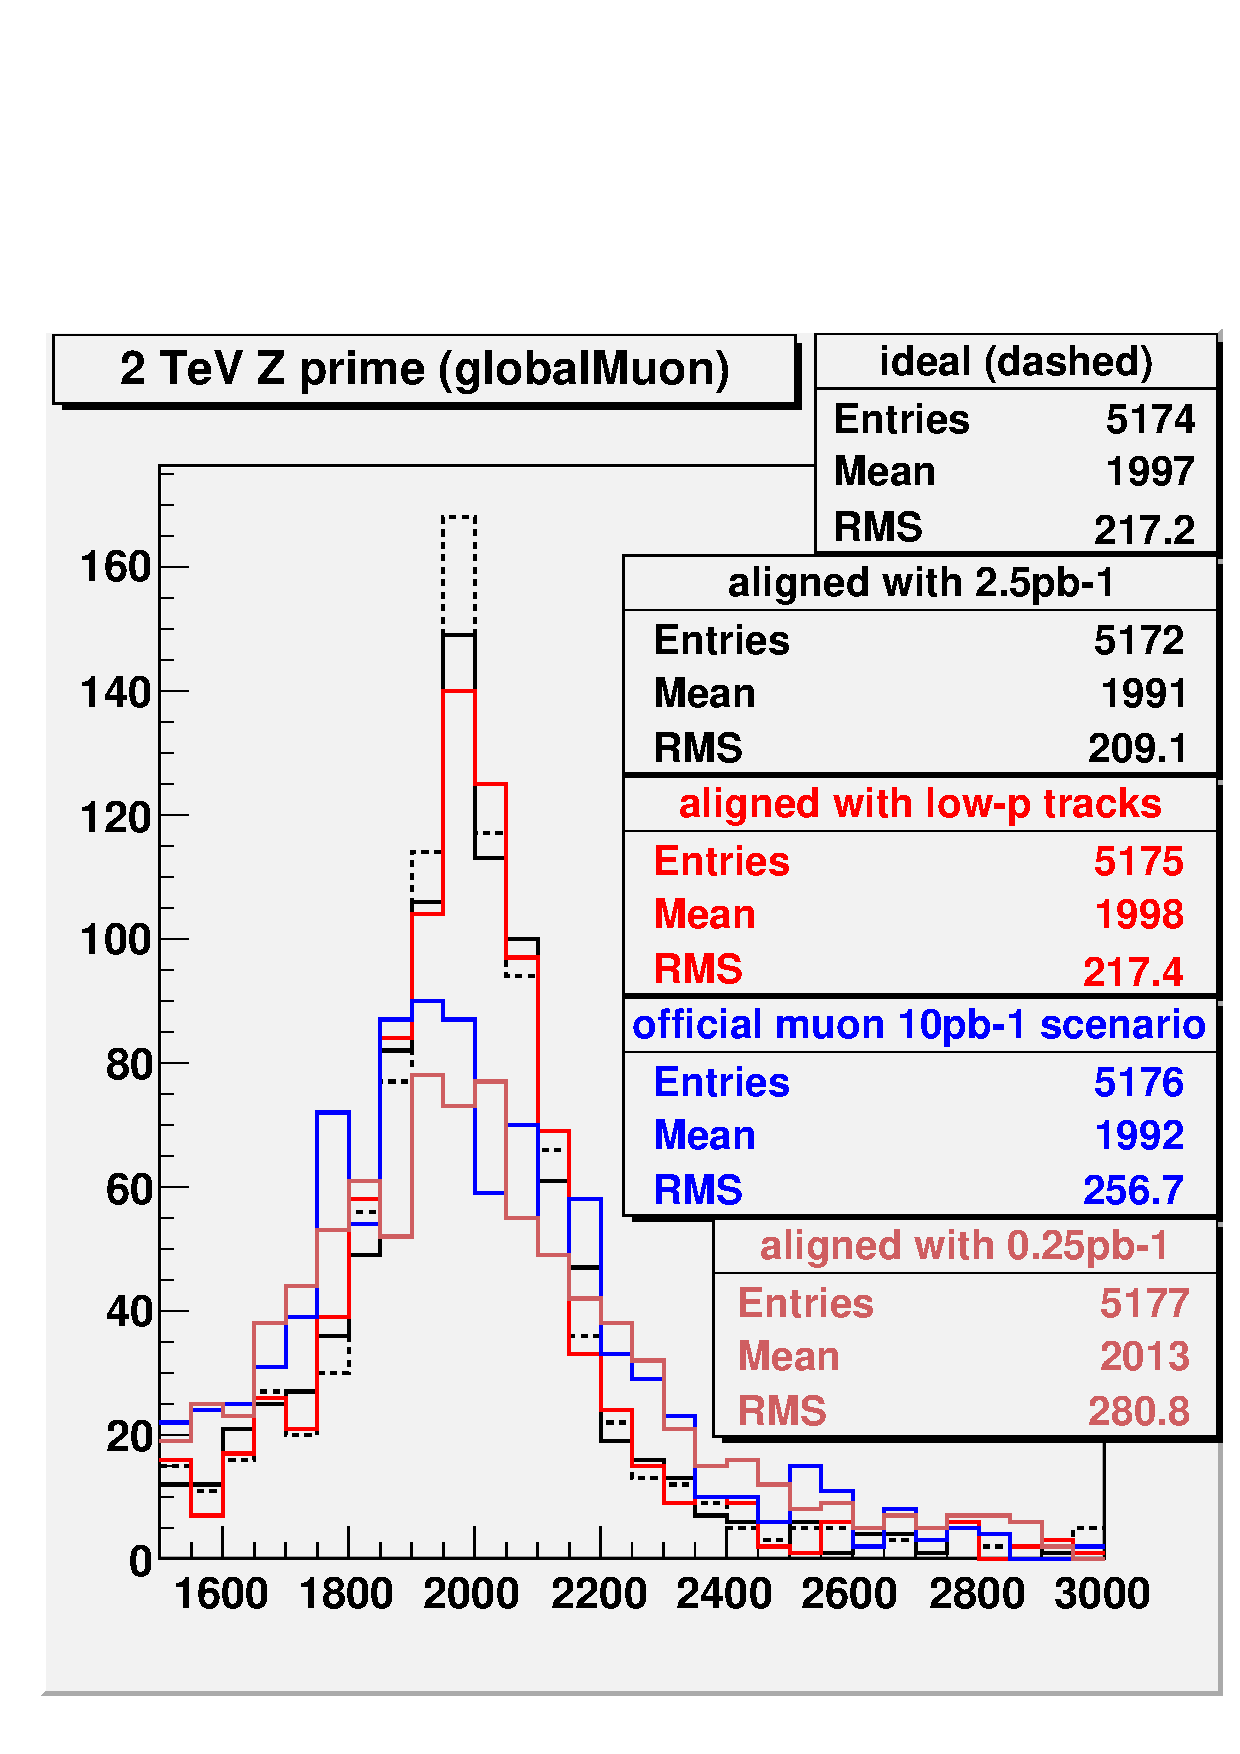
\includegraphics[width=\linewidth]{muoncompare_zprime_2000.pdf}}
\end{columns}

\vspace{0.25 cm}
\textcolor{red}{``low-p'' means 20-60~GeV $Z\to\mu\mu$}

\textcolor{blue}{official 10~pb$^{-1}$ scenario is pessimistic}
\end{frame}

\begin{frame}
\frametitle{Comparison with tracker alignment scenario}
\begin{columns}
\column{0.5\linewidth}
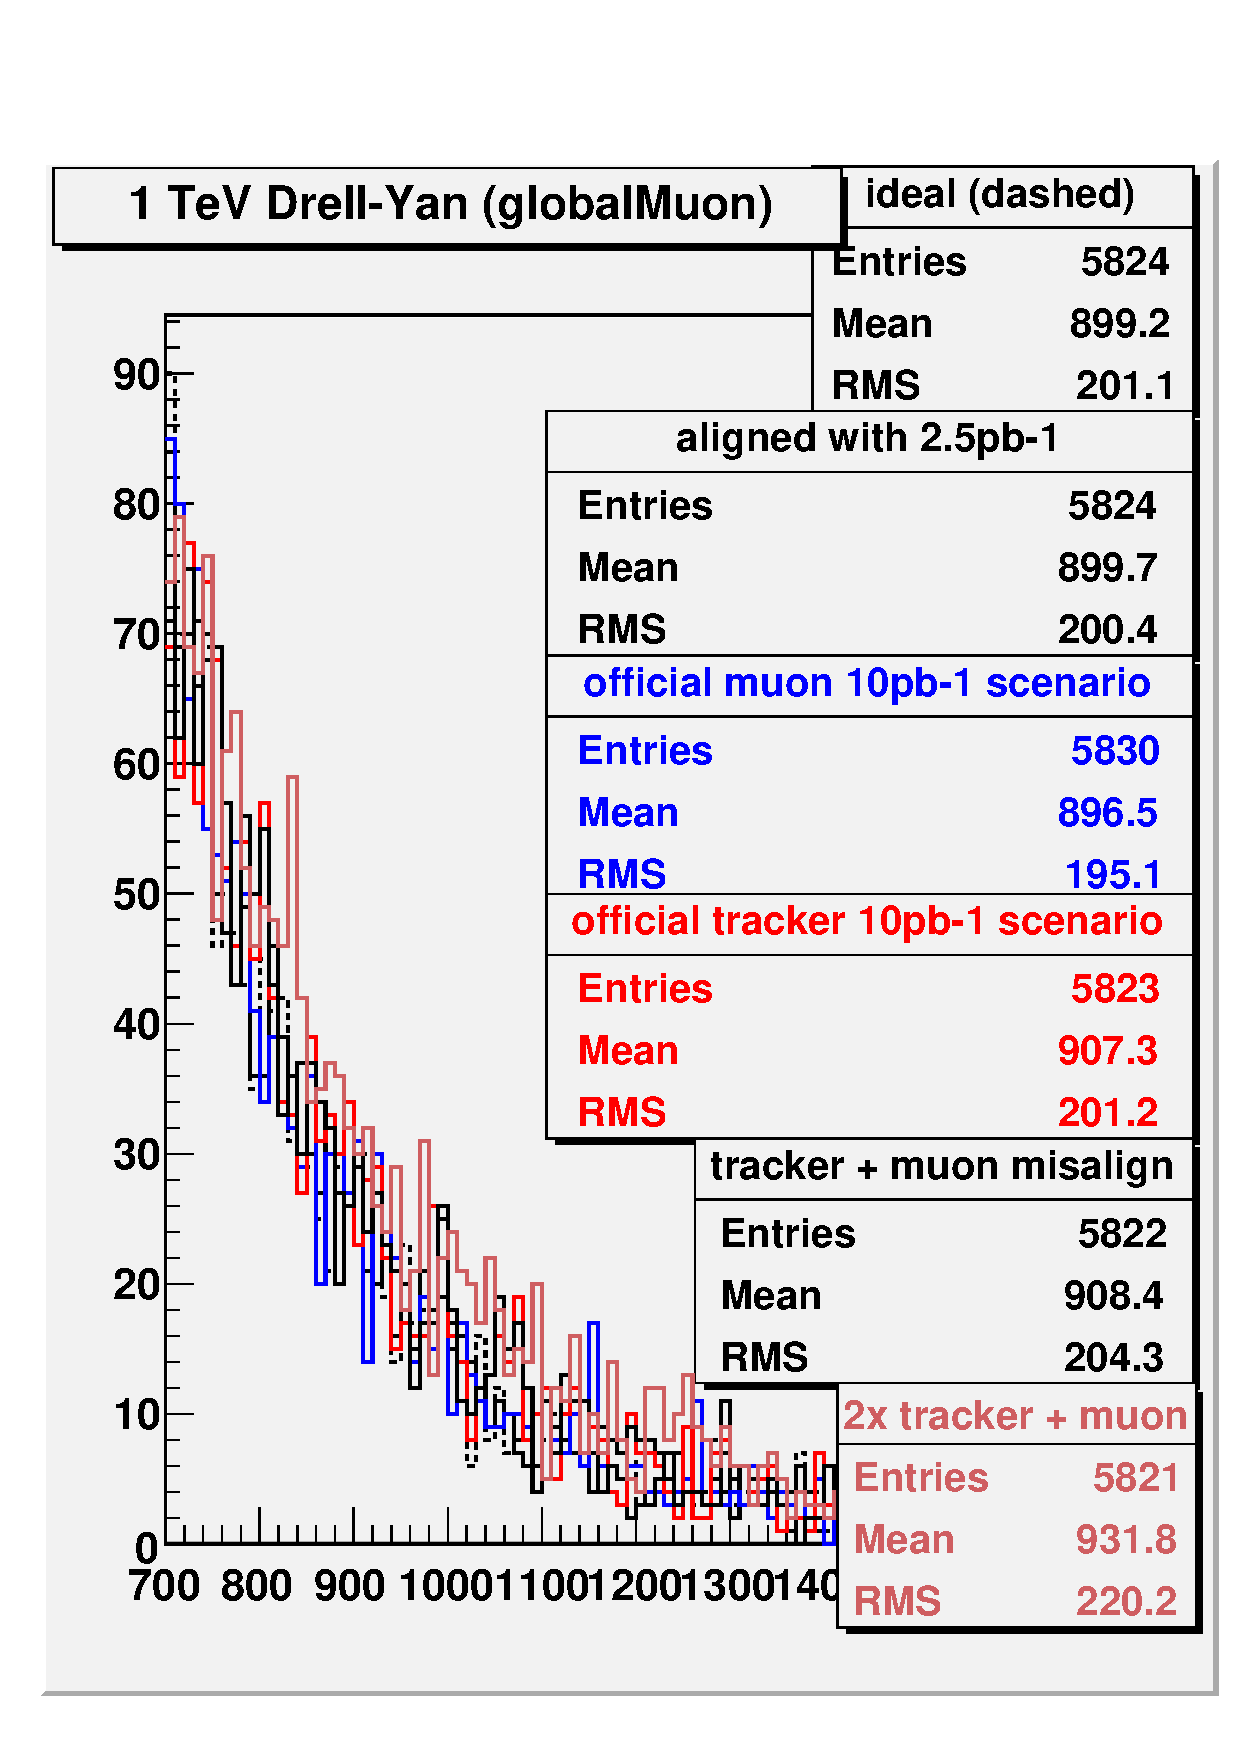
\includegraphics[width=\linewidth]{trackercompare_dy_500.pdf}
\column{0.5\linewidth}
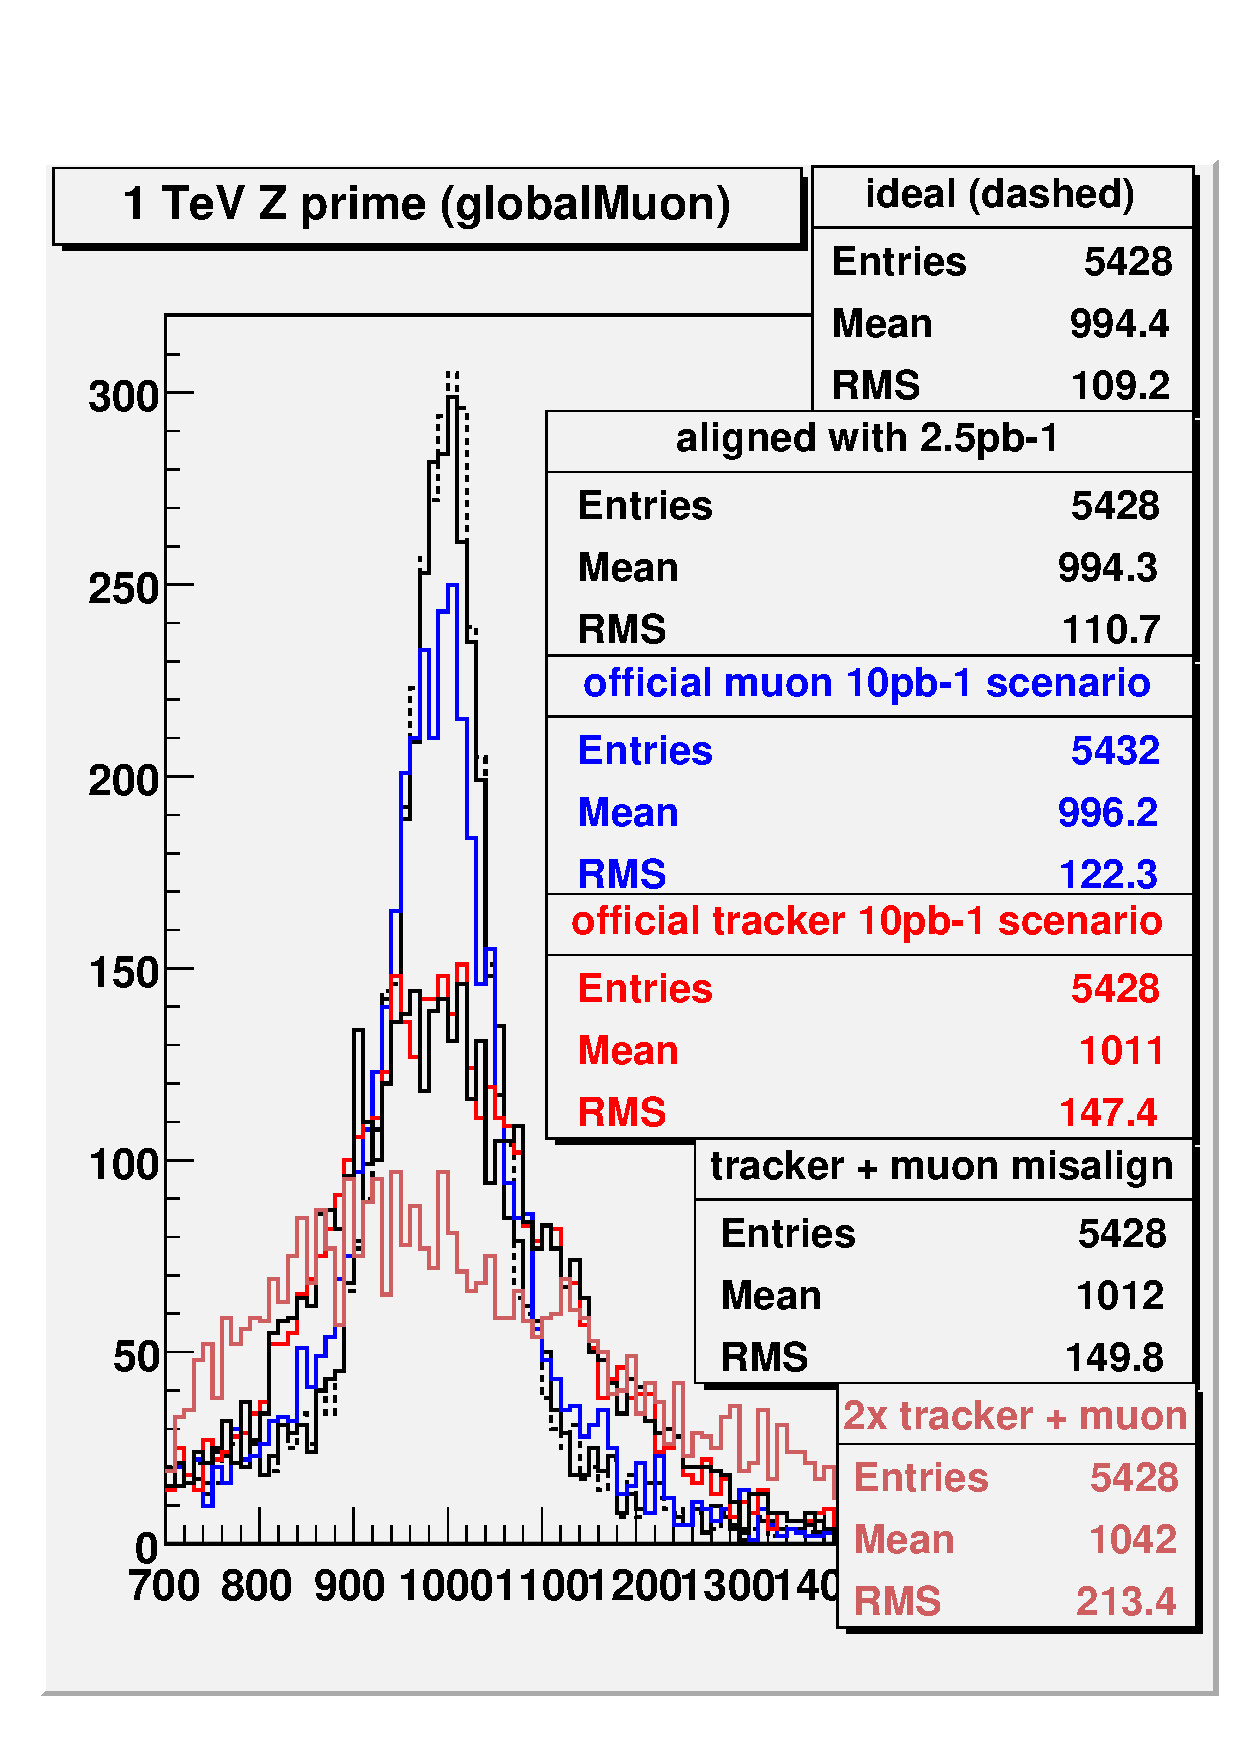
\includegraphics[width=\linewidth]{trackercompare_zprime_1000.pdf}
\end{columns}

\vspace{0.25 cm}
Careful!  Tracker alignment scenario might be pessimistic, too
\end{frame}

\begin{frame}
\frametitle{Comparison with tracker alignment scenario}
\begin{columns}
\column{0.5\linewidth}
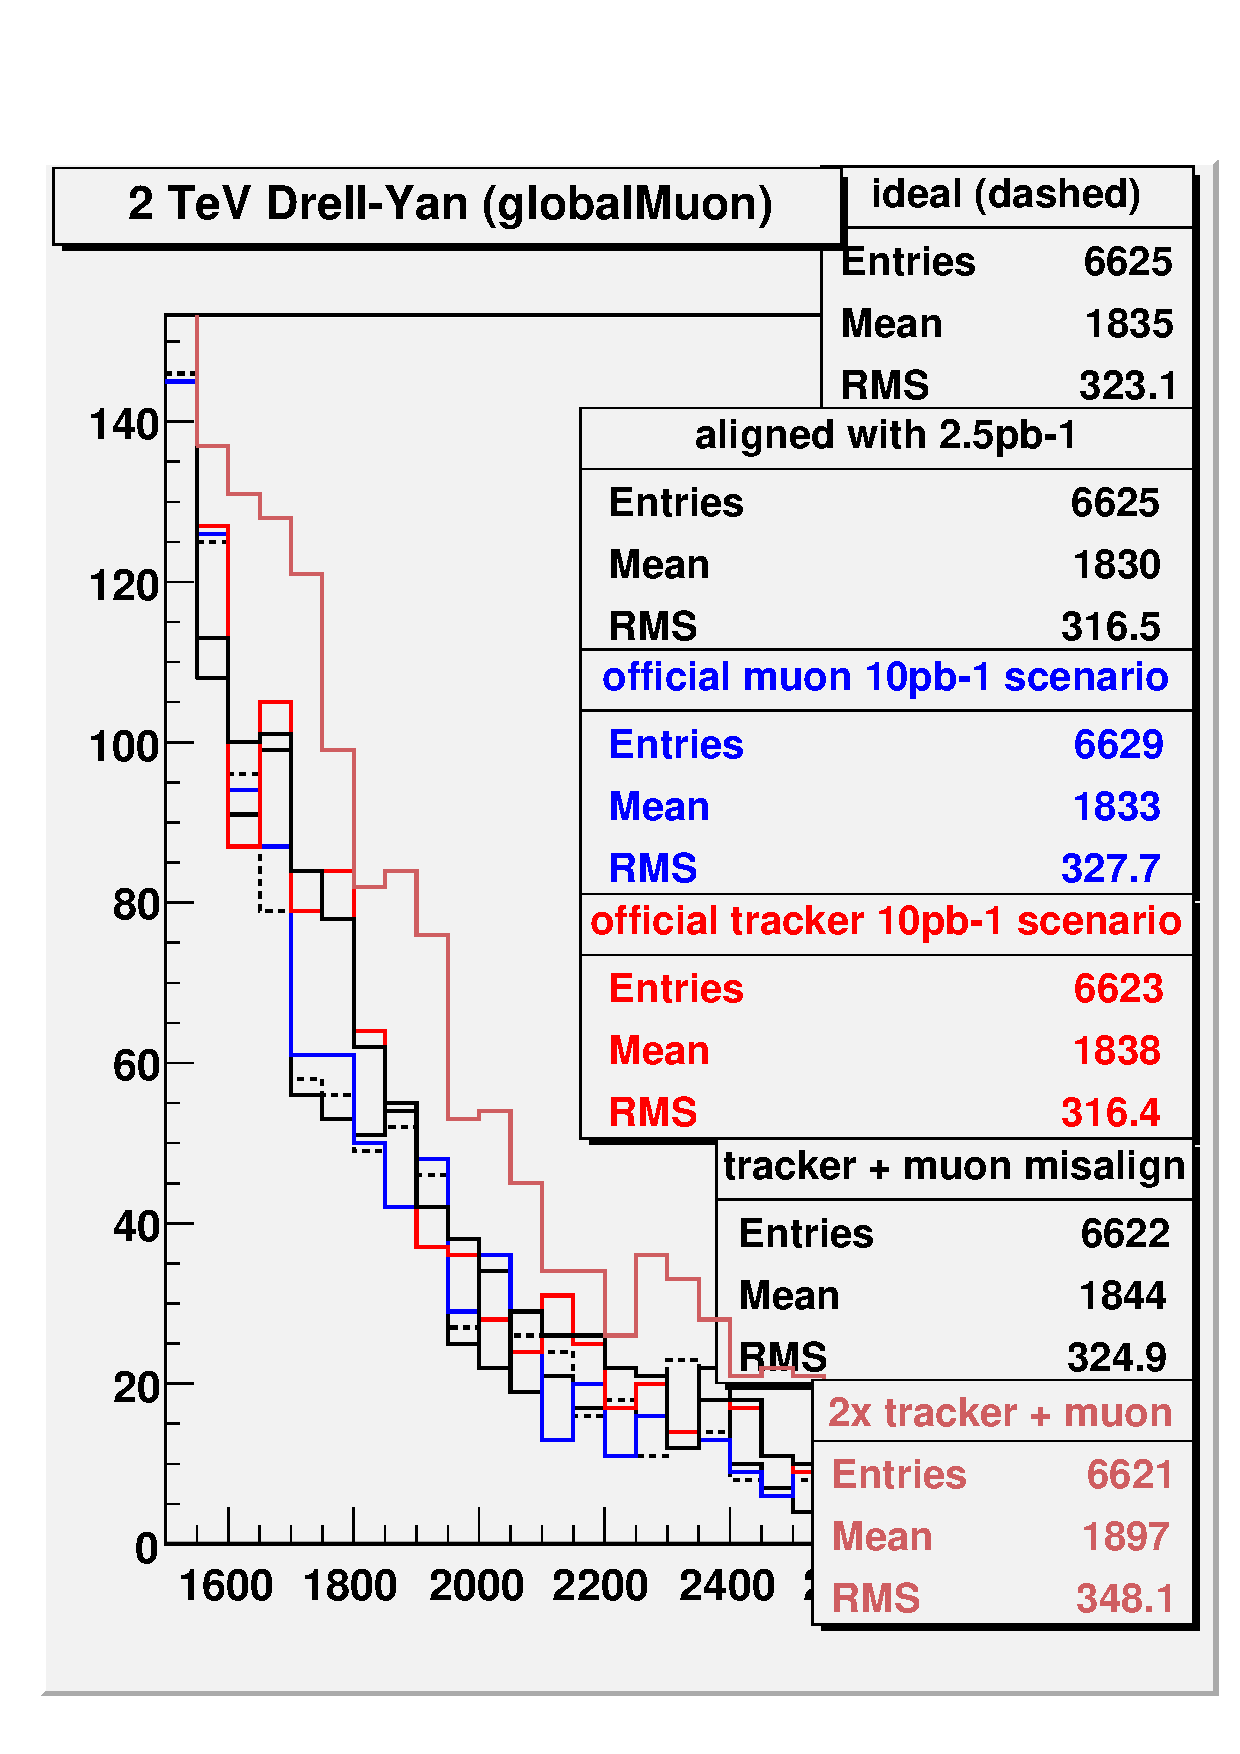
\includegraphics[width=\linewidth]{trackercompare_dy_1000.pdf}
\column{0.5\linewidth}
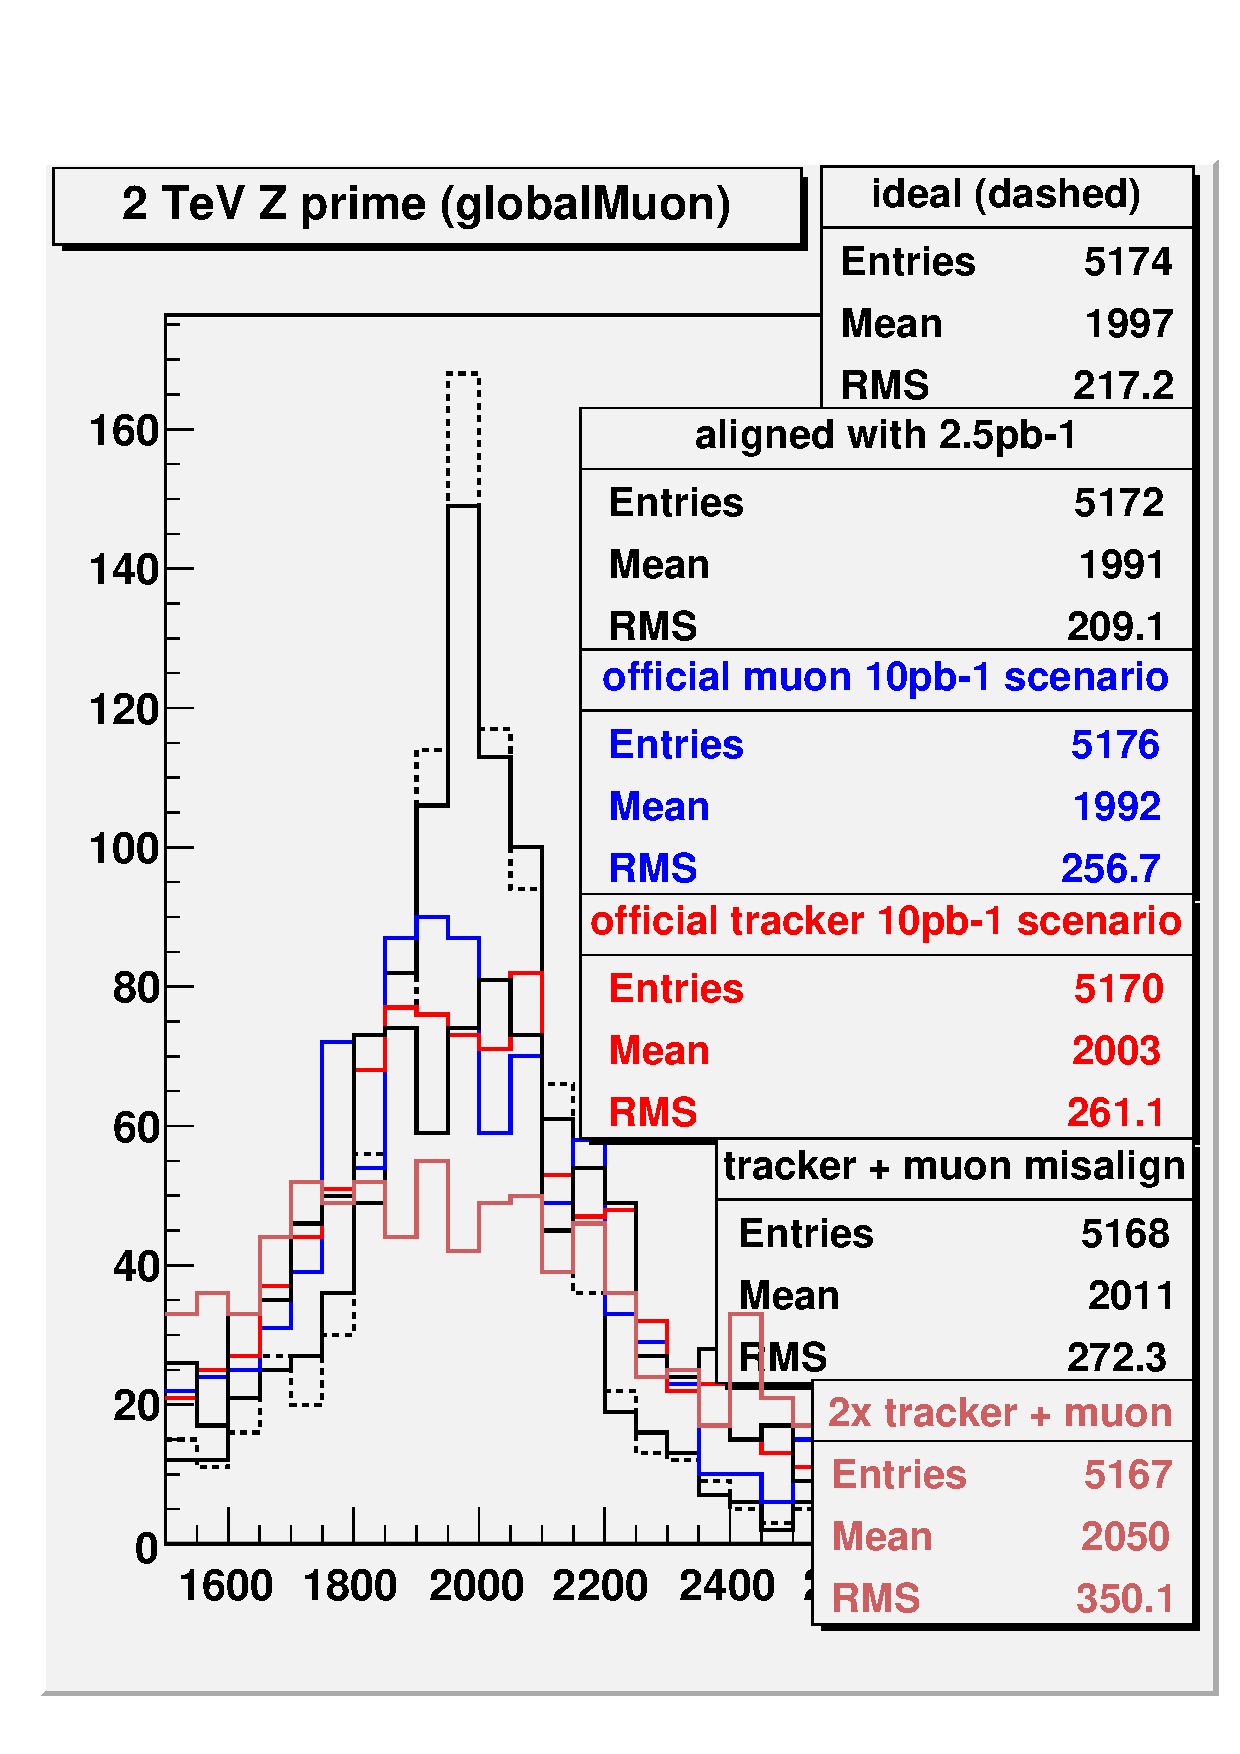
\includegraphics[width=\linewidth]{trackercompare_zprime_2000.pdf}
\end{columns}

\vspace{0.25 cm}
Careful!  Tracker alignment scenario might be pessimistic, too
\label{numpages}
\end{frame}

\begin{frame}
\frametitle{How much does a misalignment broaden di-muon mass?}
\begin{center}
RMS of event-by-event $\displaystyle \frac{\mbox{misaligned di-muon mass}}{\mbox{ideal di-muon mass}} - 1$
\end{center}

%% 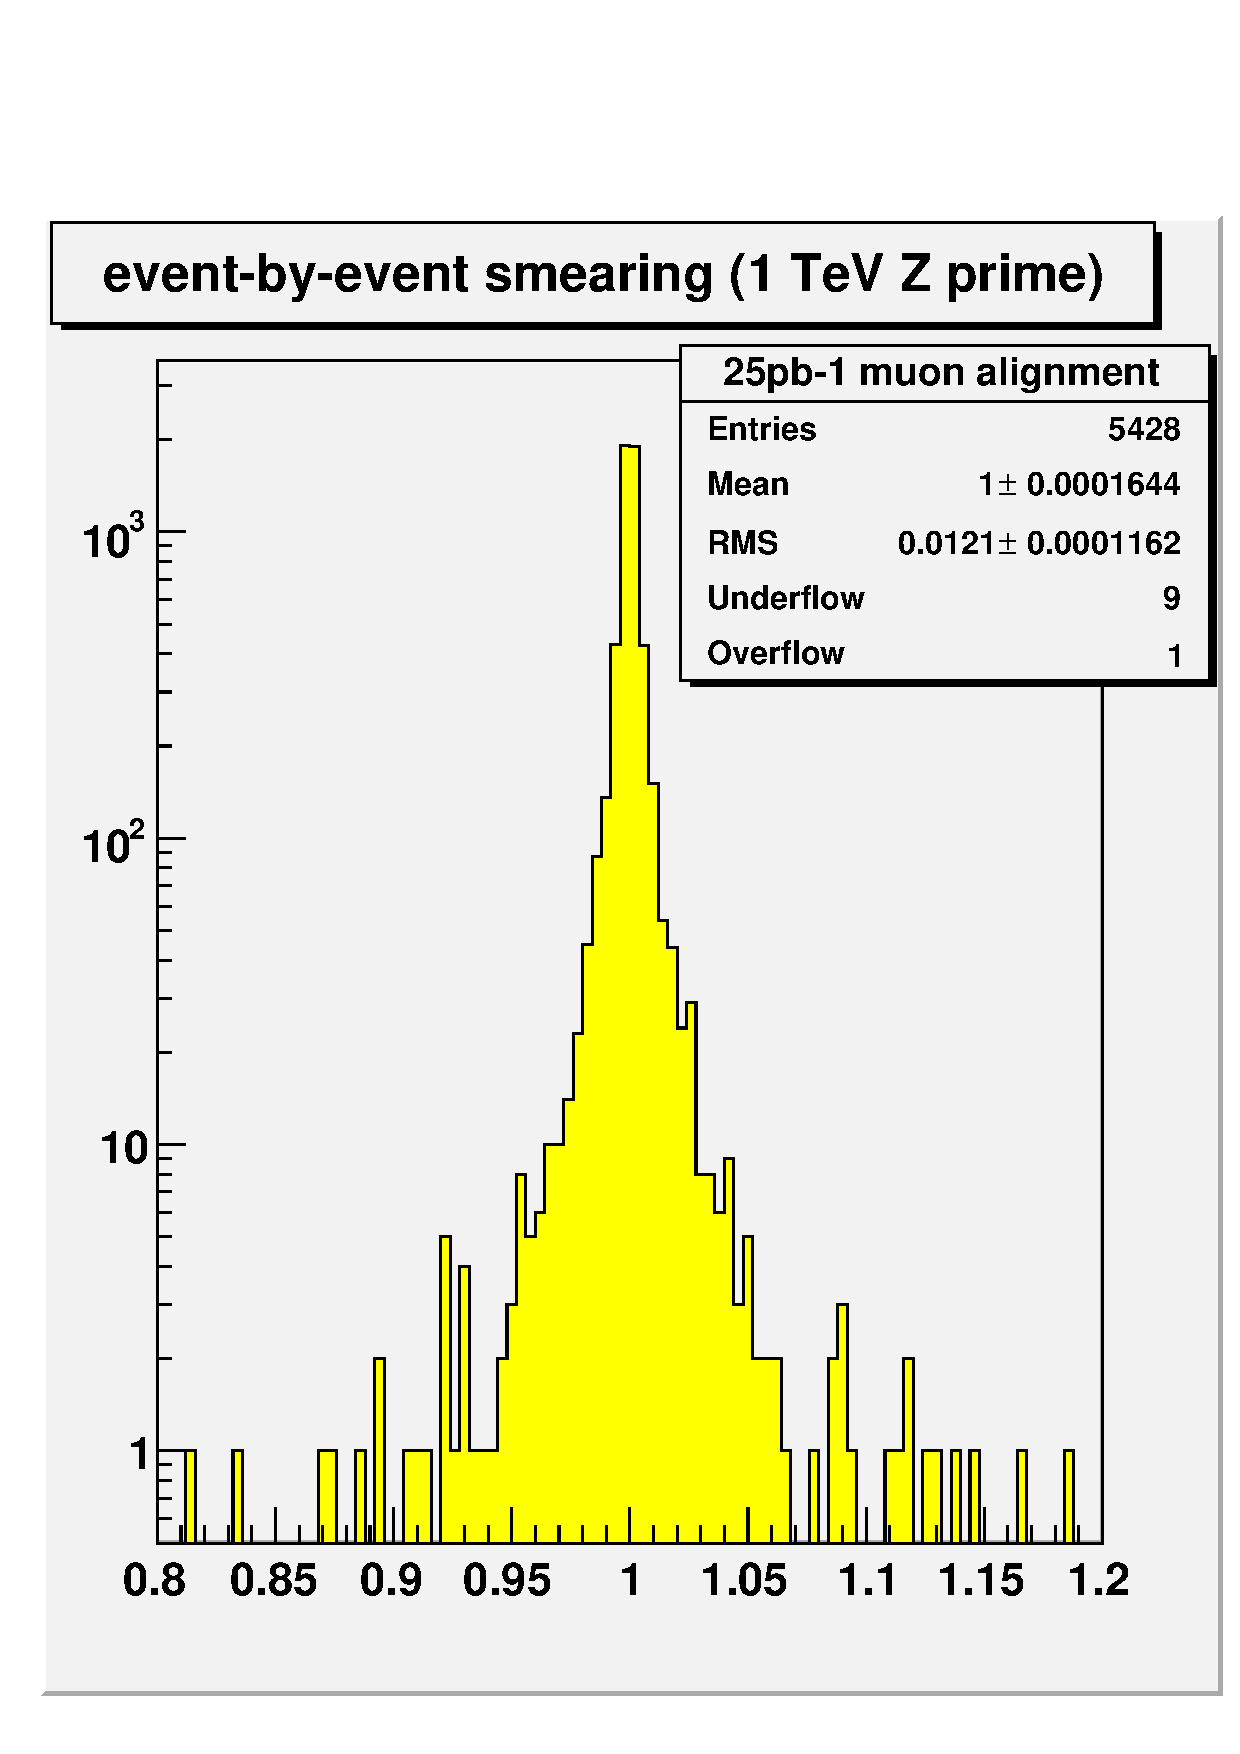
\includegraphics[width=0.25\linewidth]{smearing_events100k.pdf}
%% 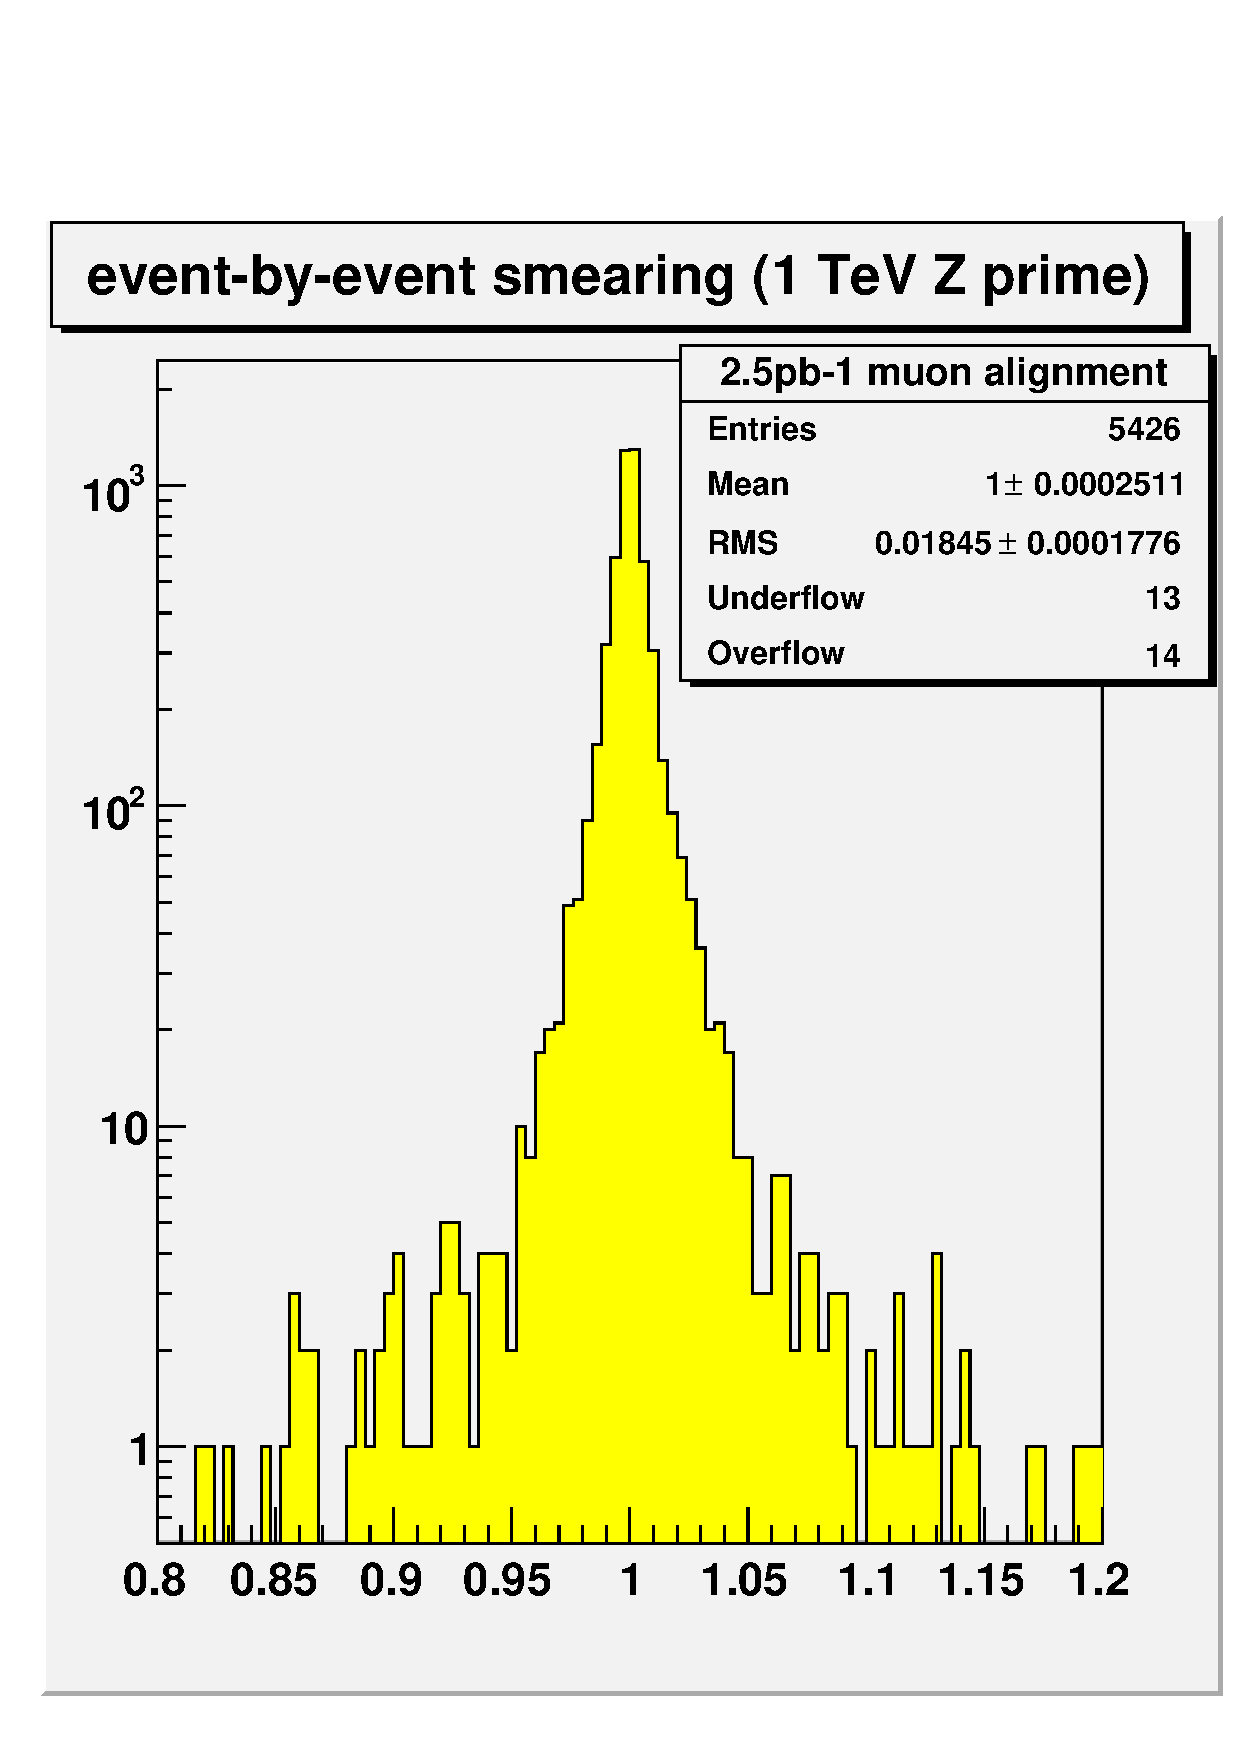
\includegraphics[width=0.25\linewidth]{smearing_events10k.pdf}
\begin{center}
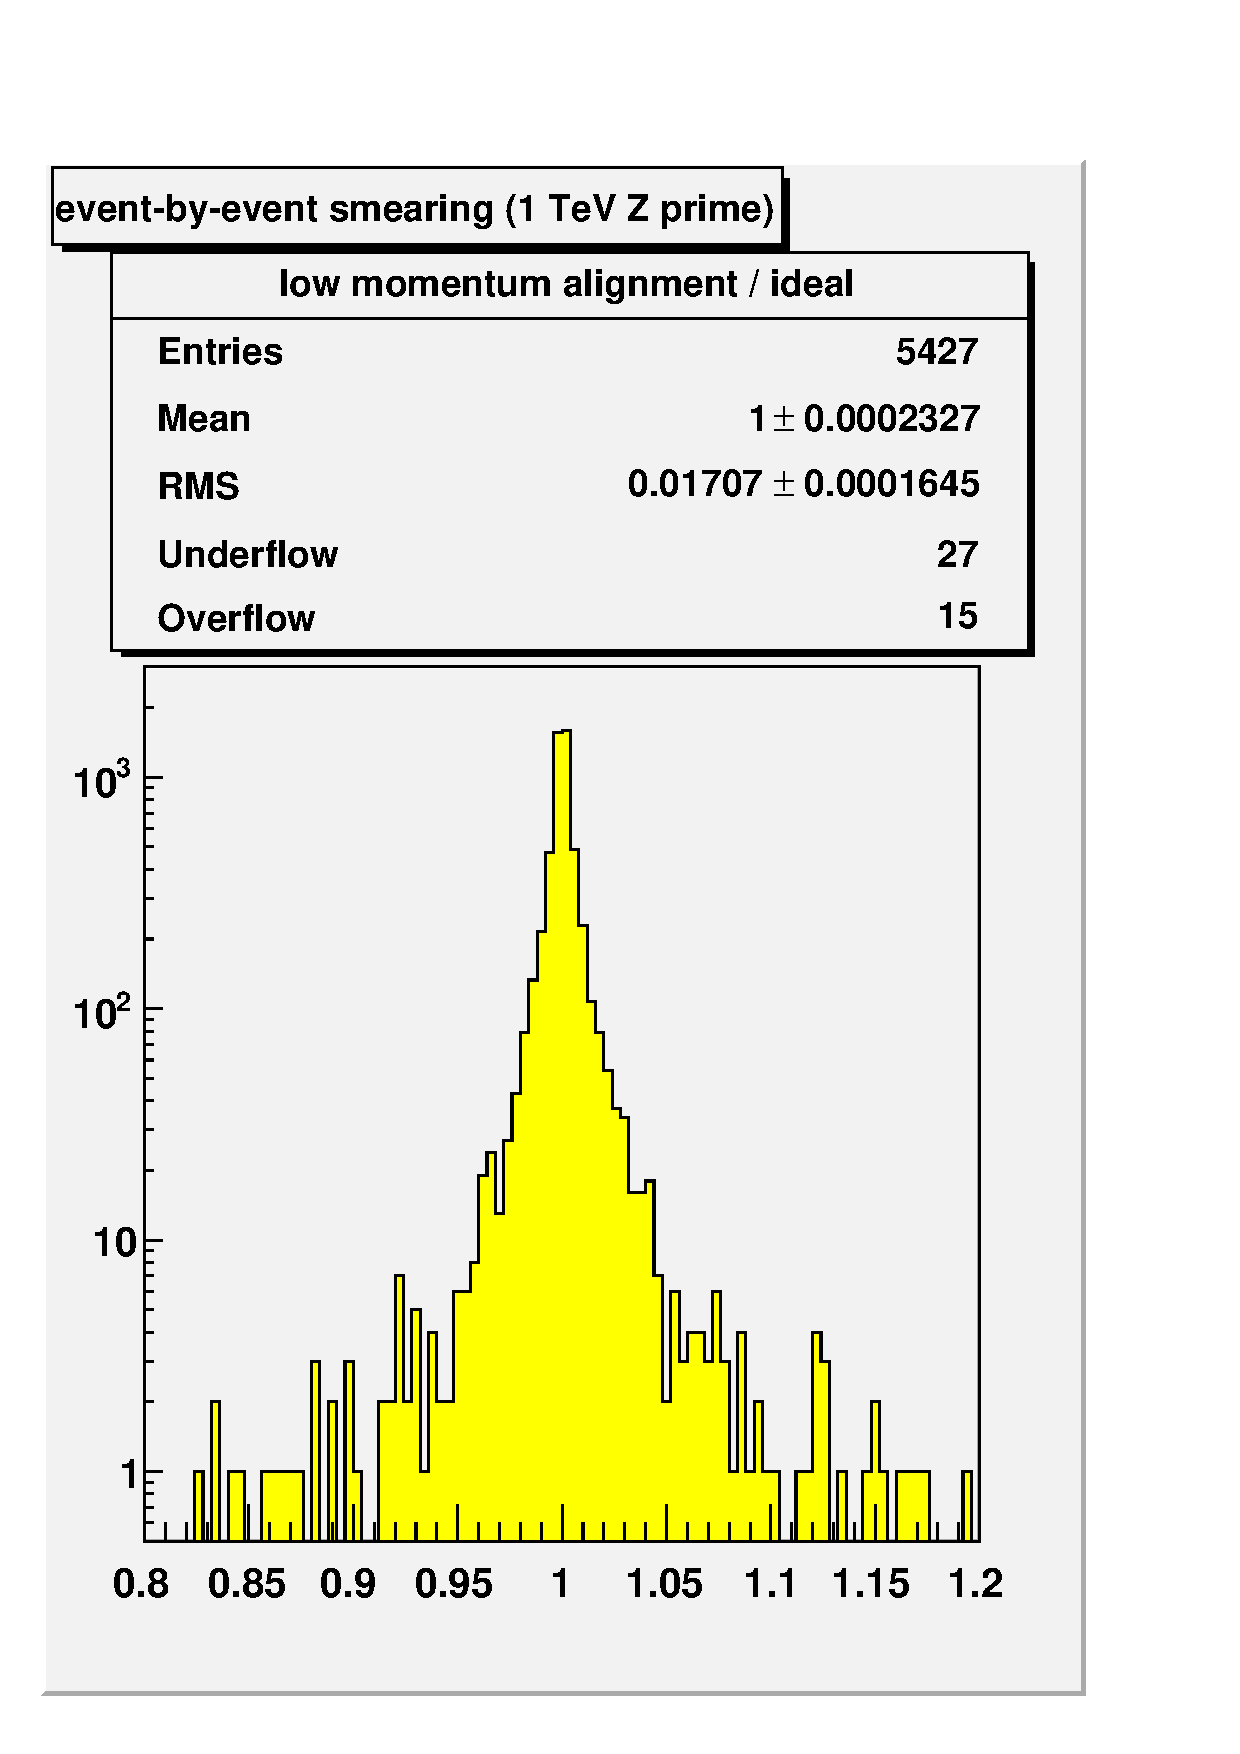
\includegraphics[width=0.35\linewidth]{smearing_momentum_low.pdf}
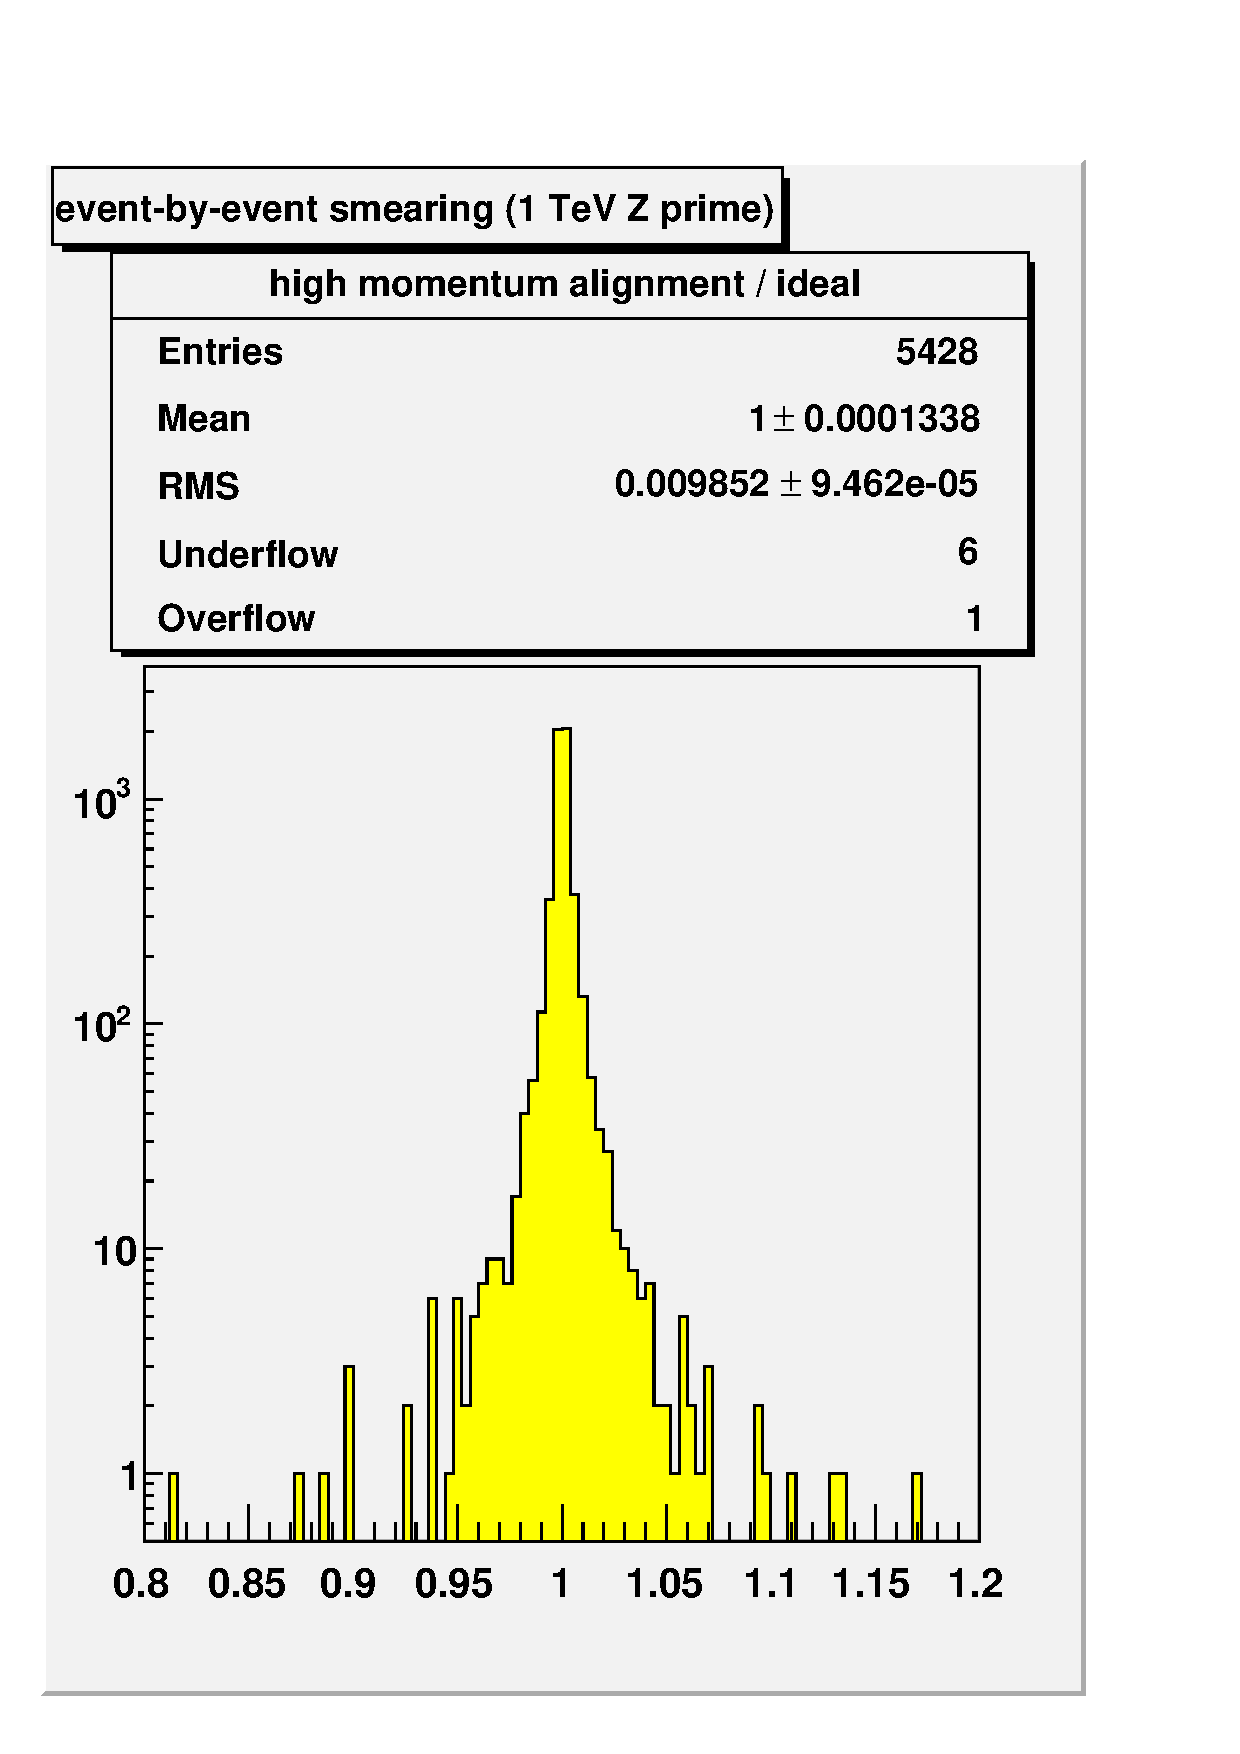
\includegraphics[width=0.35\linewidth]{smearing_momentum_high.pdf}
\end{center}

\underline{\it aligned} with: 20 $<$ $|\vec{p}|$ $<$ 60~GeV \mbox{\hspace{0.65 cm}} $|\vec{p}|$ $>$ 60~GeV \mbox{\hspace{1 cm}}~\mbox{ }
\end{frame}

\begin{frame}
\frametitle{Comparison of alignment scenarios}
\begin{center}
RMS of event-by-event $\displaystyle \frac{\mbox{misaligned di-muon mass}}{\mbox{ideal di-muon mass}} - 1$
\end{center}

\vfill
\renewcommand{\arraystretch}{1.2}
\begin{tabular}{c c c c c}
Source of alignment & $Z'$(1000) & $Z'$(2000) & DY(1000) & DY(2000) \\\hline
1k $\mu$ (0.25~pb$^{-1}$) & 6.0\% & 5.5\% & 4.8\% & 6.6\% \\
10k $\mu$ (2.5~pb$^{-1}$) & 1.8\% & 1.7\% & 1.6\% & 2.1\% \\
100k $\mu$ (25~pb$^{-1}$) & 1.2\% & 1.1\% & 1.0\% & 1.3\% \\
325k $\mu$ (82~pb$^{-1}$) & 1.0\% & 1.0\% & 0.7\% & 1.2\% \\\hline
$|\vec{p}|$ $>$ 60~GeV & 1.0\% & 1.0\% & 0.8\% & 1.2\% \\
20 $<$ $|\vec{p}|$ $<$ 60~GeV & 1.7\% & 1.7\% & 1.5\% & 2.1\%
\end{tabular}

\vfill\vfill\vfill Does not include broadening of di-muon mass due to other
detector effects (denominator is recontructed with ideal geometry, not
generator-level di-muon mass)
\end{frame}

\begin{frame}
\frametitle{Fractional widening of momentum distribution, binned}
\begin{columns}
\column{0.8\linewidth}
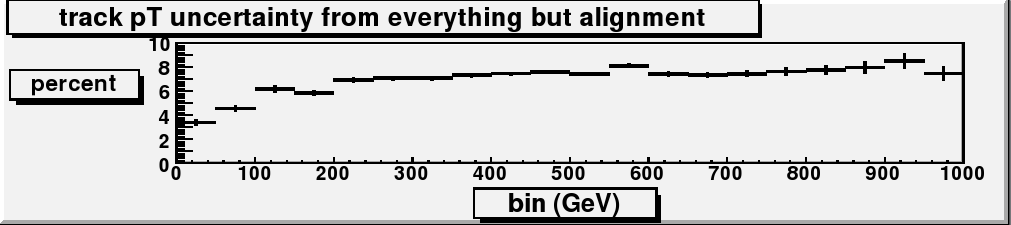
\includegraphics[width=\linewidth]{track_uncertainty_from_all_but_alignment.png}

\only<1>{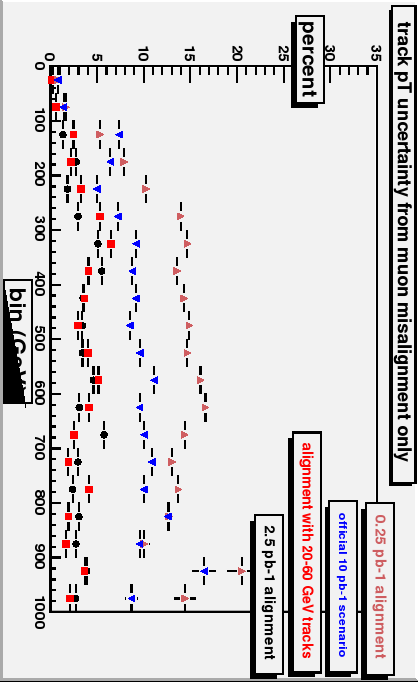
\includegraphics[height=\linewidth, angle=90]{track_uncertainty_from_muon_misalignment.png}}
\only<2>{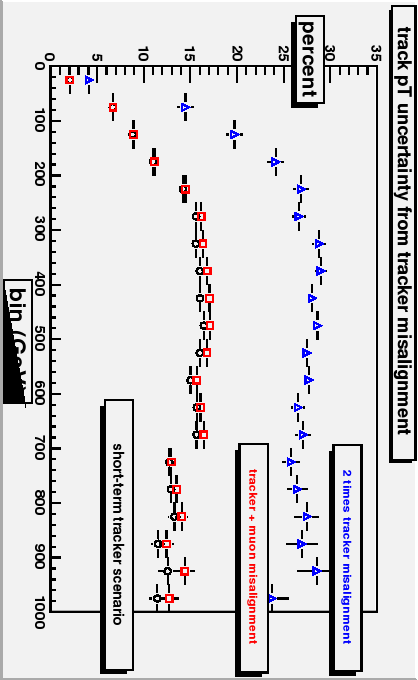
\includegraphics[height=\linewidth, angle=90]{track_uncertainty_from_tracker_misalignment.png}}

\column{0.3\linewidth}
track-by-track RMS

\vspace{0.1 cm}
of $\displaystyle \frac{{p_T}_{\mbox{\scriptsize ideal}}}{{p_T}_{\mbox{\scriptsize generated}}} - 1$

\vspace{0.75 cm}
track-by-track RMS

\vspace{0.1 cm}
of $\displaystyle \frac{{p_T}_{\mbox{\scriptsize misaligned}}}{{p_T}_{\mbox{\scriptsize ideal}}} - 1$

\vspace{1.5 cm}
$\displaystyle \bigg(\frac{\sigma_{p_T}}{p_T}\bigg) = \bigg(\frac{\sigma_\kappa}{\kappa}\bigg)$

\vspace{0.1 cm}
\mbox{$=$ sum in quadrature} \mbox{of both uncertainties}
\end{columns}
\end{frame}

\end{document}
